% Supporting Information — target-anchored antimalarial docking
\documentclass[journal=jcisd8,manuscript=suppinfo]{achemso}
\usepackage[T1]{fontenc}
\usepackage[utf8]{inputenc}
\usepackage{lmodern}
\usepackage{amsmath,amssymb,mathtools}
\usepackage[detect-all=true,group-minimum-digits=4]{siunitx}
\DeclareSIUnit\angstrom{\text{\AA}}
\DeclareSIUnit\calorie{cal}
\DeclareSIUnit\dalton{Da}
\usepackage{graphicx}
\usepackage{booktabs,tabularx,array,longtable}
\usepackage{xr}
\usepackage[colorlinks=true,linkcolor=blue,citecolor=blue,urlcolor=blue]{hyperref}
\usepackage[noabbrev,capitalize]{cleveref}
\externaldocument[M-]{Antimalarial_Candidates_African_NP_V2608}
\graphicspath{{Graphics/}}
\author{Myke Vital Sao Temgoua}
\author{Jean-Pierre Tchapet Njafa}
\author{Penabei Samafou}
\author{Wilfred Fon Mbacham}
\author{Serge Guy Nana Engo}
\title{Supporting Information: Target-Anchored Computational Prioritization of African-Natural-Product-Inspired Antimalarial Candidates}
\begin{document}

\noindent This Supporting Information documents the data, pocket definitions, docking settings, quality-control rules, and complete score matrix underlying the main article. It is organized as reproducibility material rather than as a second narrative article. The four-target panel is computational; its scores are not experimental affinities.

\section*{S1. Study design and cohort definition}
The upstream hybrid library contained \num{65856} unique molecules derived from \num{396} African natural products and \num{454} synthetic antimalarial compounds. The present target-anchored analysis used the locked 17-member Set-C polypharmacology-oriented cohort. Set A (MPO top-20) and Set B (parent-study MD top-20) were not substituted for Set C. Canonical SMILES, candidate identifiers, source hashes, and inclusion labels are provided in \texttt{results/integrated\_candidate\_manifest.csv}.

\section*{S2. Target and anchor evidence}
\begin{table}[h]
\centering
\caption{Target-specific pocket anchors and evidence classes.}
\label{tab:anchors}
\begin{tabular}{@{}llllp{5.3cm}@{}}
\toprule
Target & PDB & Anchor & Box (\si{\angstrom}) & Evidence class \\
\midrule
PfDHFR & 7F3Y & MTX A702 & 18 & Catalytic-site ligand anchor \\
PfCRT & 6UKJ & Y01 A501 & 28 & Membrane/cavity proxy; not an inhibitor \\
PfClpP & 2F6I & Ser252/His223/Asp219 & 28 & Catalytic-triad anchor \\
PfATP4 & 9N10 & D451/DPPR & 25 & Conserved machinery; no inhibitor anchor \\
\bottomrule
\end{tabular}
\end{table}

The historical 4GM2 structure is PfClpR and is excluded from PfClpP interpretation. The PfCRT and PfATP4 evidence classes are intentionally weaker than a co-crystallized small-molecule pocket and should be treated as exploratory.

\section*{S3. Ligand preparation and Vina settings}
SMILES were standardized, embedded in three dimensions, and converted to PDBQT with Meeko, following established Vina preparation conventions \cite{Trott2009,Eberhardt2021}. Each target--candidate pair used a fixed receptor and target-specific configuration. No pose was translated after docking, and no search box was expanded after inspecting a result. The geometric gate required a rank-1 centroid in the box, a minimum anchor distance no greater than \qty{10}{\angstrom}, and an in-box atom fraction of at least \qty{90}{\percent}. The full configuration and output hashes are stored with the raw result records. Because the four receptors have different pocket architectures and evidence classes, no arithmetic mean across targets is reported or used for prioritization.

\section*{S4. Complete four-target score matrix}
\begin{table}[h]
\centering
\caption{Raw Vina scoring-function estimates for the 17-member cohort. Units are \si{\kilo\calorie\per\mole}; values are not measured free energies.}
\label{tab:vina_matrix}
\small
\begin{tabular}{@{}lrrrr@{}}
\toprule
Candidate & PfDHFR & PfCRT & PfClpP & PfATP4 \\
\midrule
PP-01 & \num{-5.947} & \num{-6.483} & \num{-5.467} & \num{-6.361} \\
PP-02 & \num{-5.562} & \num{-6.124} & \num{-5.907} & \num{-6.591} \\
PP-03 & \num{-6.089} & \num{-6.633} & \num{-6.358} & \num{-7.311} \\
PP-04 & \num{-5.493} & \num{-5.329} & \num{-5.386} & \num{-6.086} \\
PP-05 & \num{-6.285} & \num{-6.412} & \num{-6.466} & \num{-6.378} \\
PP-06 & \num{-6.267} & \num{-7.907} & \num{-7.031} & \num{-7.285} \\
PP-07 & \num{-6.226} & \num{-6.633} & \num{-6.226} & \num{-5.775} \\
PP-08 & \num{-4.935} & \num{-5.213} & \num{-5.052} & \num{-5.494} \\
PP-09 & \num{-5.693} & \num{-6.871} & \num{-5.613} & \num{-6.078} \\
PP-10 & \num{-6.346} & \num{-6.395} & \num{-6.016} & \num{-6.670} \\
PP-11 & \num{-6.179} & \num{-6.376} & \num{-6.583} & \num{-6.724} \\
PP-12 & \num{-5.248} & \num{-6.357} & \num{-5.386} & \num{-4.635} \\
PP-13 & \num{-5.921} & \num{-5.685} & \num{-6.454} & \num{-7.565} \\
PP-14 & \num{-4.863} & \num{-5.328} & \num{-5.047} & \num{-5.460} \\
PP-15 & \num{-6.045} & \num{-6.084} & \num{-6.366} & \num{-7.016} \\
PP-16 & \num{-5.469} & \num{-6.202} & \num{-6.203} & \num{-6.451} \\
PP-17 & \num{-5.266} & \num{-5.116} & \num{-5.342} & \num{-5.360} \\
\bottomrule
\end{tabular}
\end{table}

\section*{S5. Per-pair geometric quality control}
All \num{68} pairs passed the computational gate. Anchor-distance ranges were \qtyrange{2.00}{3.79}{\angstrom} for PfDHFR, \qtyrange{3.03}{4.08}{\angstrom} for PfCRT, \qtyrange{3.29}{8.88}{\angstrom} for PfClpP, and \qtyrange{1.98}{3.79}{\angstrom} for PfATP4. These values describe pose placement relative to the declared anchors; they do not measure residence time, binding kinetics, or biological engagement.

\begin{figure}[htbp]
\centering
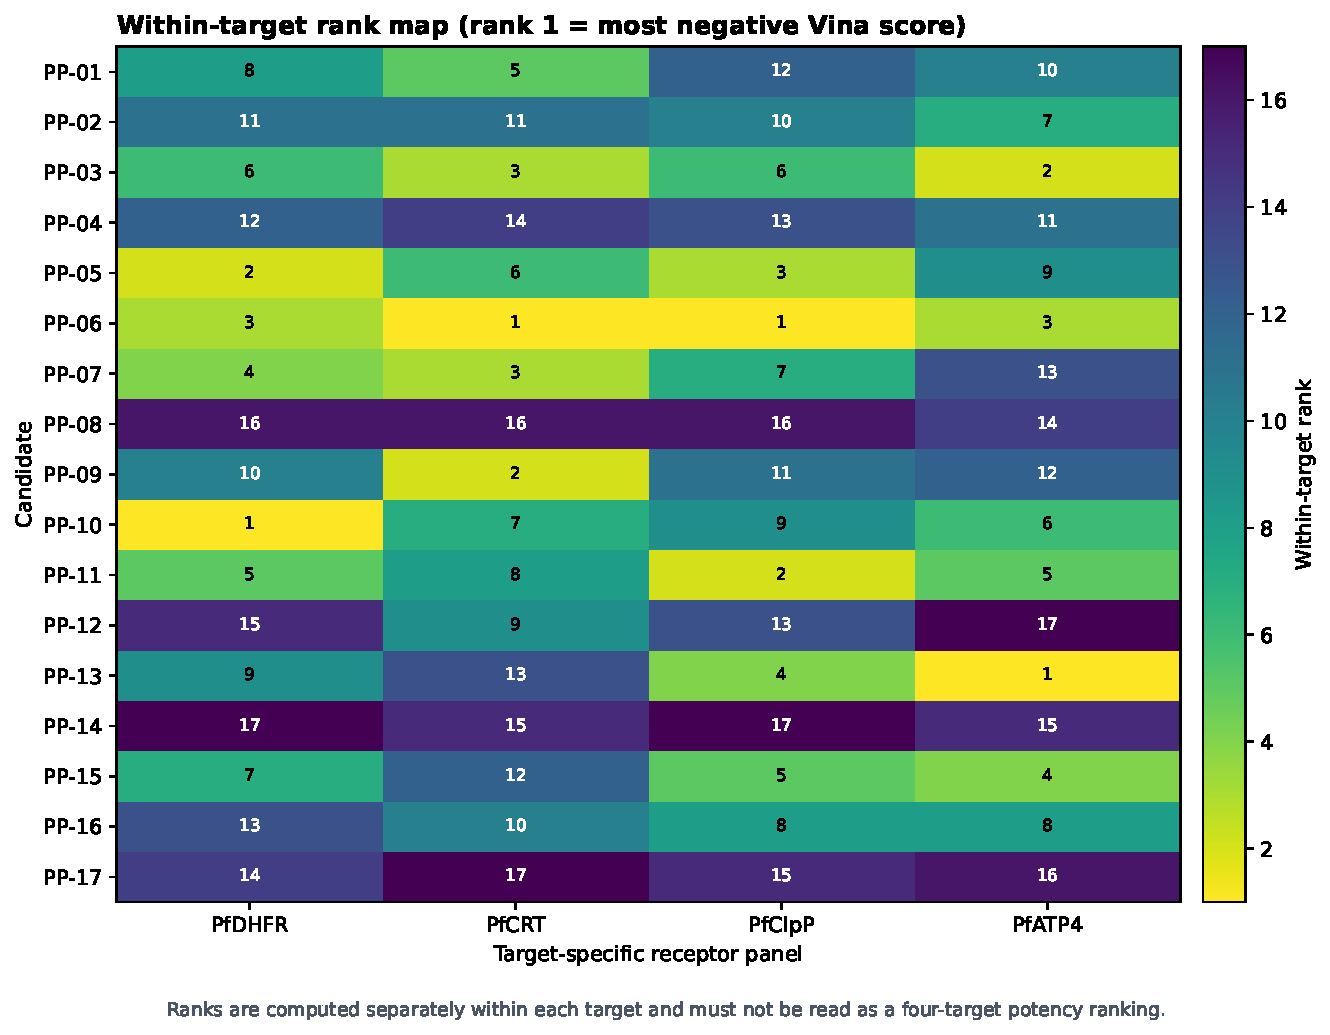
\includegraphics[width=0.95\textwidth]{p1_v5_intratarget_rank_heatmap.pdf}
\caption{Within-target rank map for the 17 candidates. Rank 1 denotes the most negative Vina score within a target; ranks are calculated independently for each receptor and must not be interpreted as a cross-target potency order. These checks assess pose placement and provenance; they are not biological validation.}
\label{fig:rank}
\end{figure}

\begin{figure}[htbp]
\centering
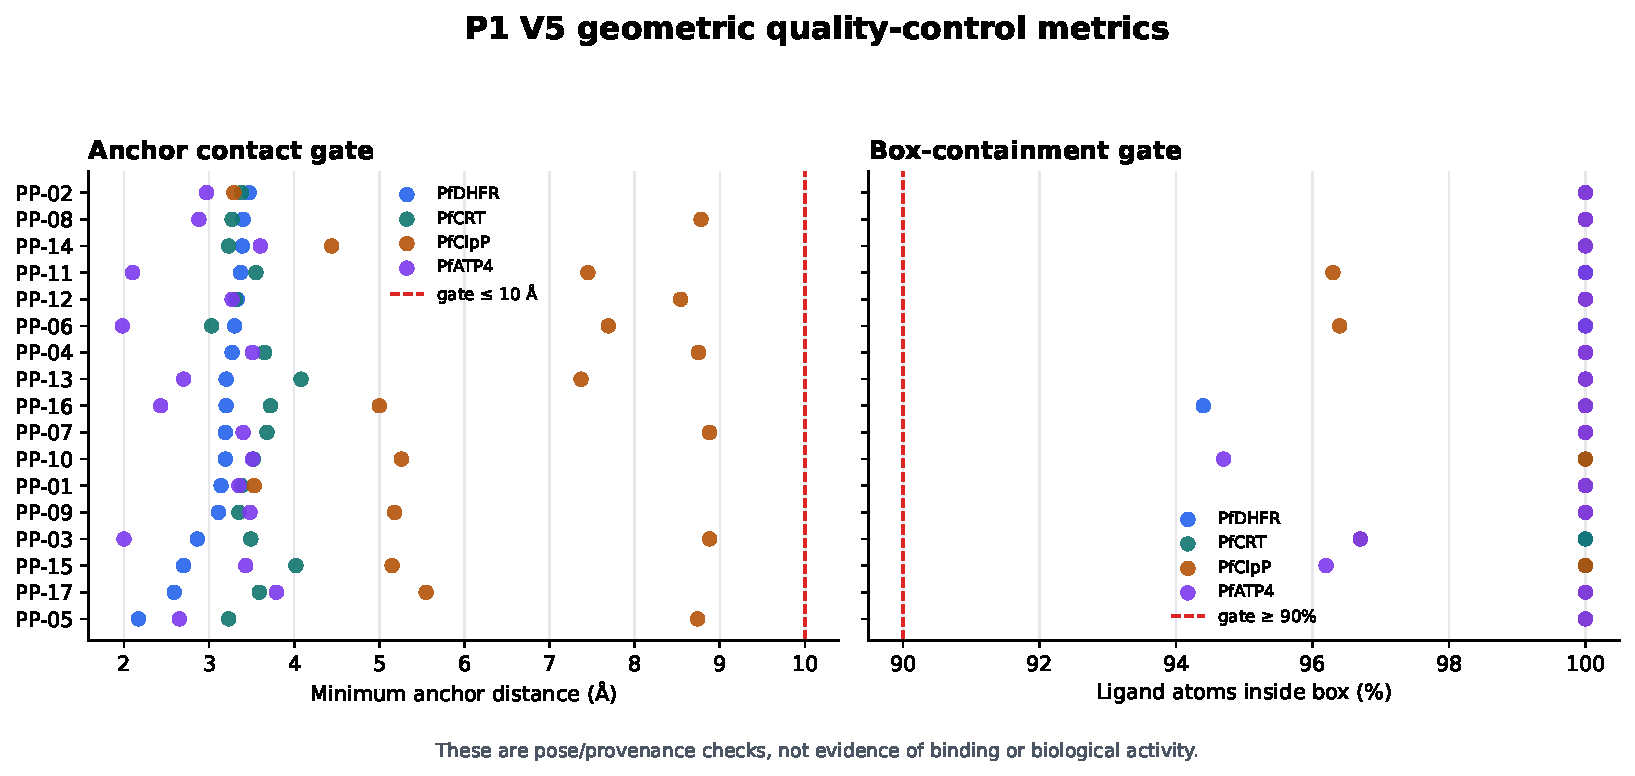
\includegraphics[width=0.95\textwidth]{p1_v5_geometric_gate_qc.pdf}
\caption{Geometric quality-control metrics for the 68 candidate--target poses. Dashed lines mark the predeclared anchor-distance and in-box-fraction thresholds. These checks assess pose placement and provenance, not binding or biological activity. These checks assess pose placement and provenance; they are not biological validation.}
\label{fig:qc}
\end{figure}

\section*{S6. What is and is not inferred}
The target-anchored panel supports a reproducible computational ranking layer. It does not support claims of confirmed inhibitors, measured IC\textsubscript{50}/EC\textsubscript{50}, resistance circumvention, or equivalent pocket validity across targets. Raw hashes and automated integrity checks document reproducibility; they do not substitute for structural or experimental validation.

\section*{S7. Data and code availability}
Raw poses, receptor and ligand files, configuration files, candidate manifests, and analysis scripts are available at \url{https://github.com/NanaEngo/Malaria_codesV2}. The four-target machine-readable table is \texttt{results/v5\_four\_target\_vina\_affinities.csv}; the per-pair review table is \texttt{results/v5\_four\_target\_vina\_review\_table.json}.

\bibliography{../bibliography/Sao_Chim_Space}
\end{document}
